%%%%%%%%%%%%%%%%%%%%%%%%%%%%%%%%%%%%%%%%%
% Memo
% LaTeX Template
% Version 1.0 (30/12/13)
%
% This template has been downloaded from:
% http://www.LaTeXTemplates.com
%
% Original author:
% Rob Oakes (http://www.oak-tree.us) with modifications by:
% Vel (vel@latextemplates.com)
%
% License:
% CC BY-NC-SA 3.0 (http://creativecommons.org/licenses/by-nc-sa/3.0/)
%
%%%%%%%%%%%%%%%%%%%%%%%%%%%%%%%%%%%%%%%%%

\documentclass[letterpaper,11pt]{texMemo} % Set the paper size (letterpaper, a4paper, etc) and font size (10pt, 11pt or 12pt)

\usepackage{fancyhdr}
\usepackage{fancybox}
\usepackage{longtable}
\usepackage{amsmath}
%----------------------------------------------------------------------------------------
%	MEMO INFORMATION
%----------------------------------------------------------------------------------------



\memoto{Luis Andr\'es Valido Fajardo. luis.valido@umcc.cu (53694742)} % Recipient(s)

\memofrom{Josval Díaz Blanco} % Sender(s)

\memosubject{Guía de Aprendizaje para Concursantes ICPC y IOI: Búsqueda Binaria } % Memo subject

\memodate{\today} % Date, set to \today for automatically printing todays date

\logo{
\includegraphics[scale=0.5]{img/icpc}} % Institution logo at the top right of the memo, comment out this line for no logo

%----------------------------------------------------------------------------------------

\titleguide{Detección de ciclos en un grafo}%all_longest_paths_tree

\begin{document}

%\AddToShipoutPicture{\BackgroundPic}
\maketitle % Print the memo header information
%\tableofcontents
\pagestyle{plain}
\pagebreak

\pagestyle{fancy}
\fancyhead[LO,CE]{ }
\fancyhead[RO,CE]{
\includegraphics[scale=0.1]{img/icpc}}
\fancyfoot[LO,CE]{\textbf{Autor:} Luis Andrés Valido Fajardo \\ \textbf{Email:} luis.valido1989@gmail.com \\ \textbf{Teléfono:} 53694742}
\fancyfoot[RO,CE]{\emph{Existen 10 tipos de personas Las que \\saben binario y LAS QUE NO}}
\fancypagestyle{plain}{\pagestyle{fancy}}



%\lhead{ }
%\rhead{  }

%\fancyfoot[L]{}
%\fancyfoot[R]{\textbf{Autor:} Luis Andrés Valido Fajardo \\ \textbf{Email:} luis.valido@umcc.cu}
%----------------------------------------------------------------------------------------
%	MEMO CONTENT
%----------------------------------------------------------------------------------------


\section{Introducción}
Considere un grafo dirigido o no dirigido sin bucles ni aristas múltiples. Tenemos que comprobar si es acíclico y, si no lo es, encontrar cualquier ciclo. Considere un gráfico sucesor que solo contiene una ruta que termina en un ciclo. Nosotros podemos plantearnos las siguientes preguntas: si comenzamos nuestra caminata en el nodo inicial, ¿Cuál es el primer nodo del ciclo y cuántos nodos contiene el ciclo?

Por ejemplo, en el grafo:

% TODO: \usepackage{graphicx} required
\begin{figure}[h!]
	\centering
	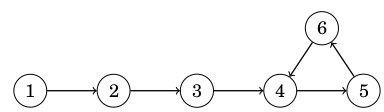
\includegraphics[width=0.7\linewidth]{img/cycle_detection}
	\label{fig:cycledetection}
\end{figure}


Si comenzamos nuestra caminata en el nodo 1, el primer nodo que pertenece al ciclo es el nodo 4,
y el ciclo consta de tres nodos (4, 5 y 6). De como detectar la existencia o no de un ciclo en grafo de acuerdo a su tipo tratará la siguiente guía.
\section{Conocimientos previos}
\subsection{Grafo dirigido}

Un grafo dirigido o digrafo es un tipo de grafo en el cual las aristas tienen un sentido definido, a 
diferencia del grafo no dirigido, en el cual las aristas son relaciones simétricas y no apuntan en ningún 
sentido.

\subsection{Grafo no dirigido}

Un grafo no dirigido es un tipo de grafo en el cual las aristas representan relaciones simétricas y no tienen un sentido definido, a diferencia del grafo dirigido, en el cual las aristas tienen un sentido y por tanto no son necesariamente simétricas. 
\section{Desarrollo}
Para explicar como realizar una detección de ciclo dentro un grafo lo primero que haremos será dividir el problema en dos, de esta forma veremos el problema para grafos dirigidos y para grafos no dirigidos de forma separada.

\subsection{Grafo dirigido}

Para resolver este problema sobre un grafo no dirigido ejecutaremos una serie de DFS en el grafo. Inicialmente todos los vértices están coloreados de blanco (0). Desde cada vértice $v$ no visitado (blanco), iniciaremos el DFS, marcamos el nodo $v$ en gris (1) al entrar en el DFS cuando se procesa  y lo marcamos en negro (2) al salir. Si DFS se mueve a un vértice gris $u$, entonces hemos encontrado un ciclo que comenzó el nodo $u$ término en el nodo $v$. El ciclo en sí se puede reconstruir utilizando un arreglo donde se almacene para cada nodo $v$ su padre. Para dicha reconstrucción empezariamos en el nodo $v$ hasta llegar al nodo $u$ apoyados en el arreglo de padres.



\subsection{Grafo no dirigido}

La solución para grafos no dirigidos es similar a los grafos dirigidos solo se debe tener en cuenta que en la versión no dirigida, si un vértice $v$ se colorea de negro, el DFS nunca volverá a visitarlo. Esto se debe a que ya exploramos todas las aristas conectadas de $v$ cuando lo visitamos por primera vez. El componente conectado que contiene $v$ (después de eliminar la arista entre $v$ y su padre) debe ser un árbol, si el DFS ha completado el procesamiento de $v$ sin encontrar un ciclo. Así que ni siquiera necesitamos distinguir entre estados grises y negros. Por lo tanto, podemos convertir el color del vector char en un vector booleano visitado.



\section{Implementación}
\subsection{C++}

\subsubsection{Grafo dirigido}
\begin{lstlisting}[language=C++]
int n;
vector<vector<int>> adj;
vector<char> color;
vector<int> parent;
int cycle_start, cycle_end;

bool dfs(int v) {
   color[v] = 1;
   for (int u : adj[v]) {
      if (color[u] == 0) {
         parent[u] = v;
         if (dfs(u)) return true;
      } else if (color[u] == 1) {
         cycle_end = v; cycle_start = u;
         return true;
      }
   }
   color[v] = 2;
   return false;
}

void find_cycle() {
   color.assign(n, 0); parent.assign(n, -1);
   cycle_start = -1;
	
   for (int v = 0; v < n; v++) {
      if (color[v] == 0 && dfs(v)) break;
   }
	
   if (cycle_start == -1) { cout << "Aciclico" << endl;} 
   else {
      vector<int> cycle;
      cycle.push_back(cycle_start);
      for (int v = cycle_end; v != cycle_start; v = parent[v])
      cycle.push_back(v); cycle.push_back(cycle_start);
      reverse(cycle.begin(), cycle.end());
      cout << "Ciclo encontrado: ";
      for (int v : cycle) cout << v << " ";
      cout << endl;
   }
}
\end{lstlisting}


\subsubsection{Grafo no dirigido}
\begin{lstlisting}[language=C++]
int n;
vector<vector<int>> adj;
vector<bool> visited;
vector<int> parent;
int cycle_start, cycle_end;

bool dfs(int v, int par) { //pasando el vertice y su vertice padre
   visited[v] = true;
   for (int u : adj[v]) {
      if (u == par) continue; // arista al vertice padre
      if (visited[u]) {
         cycle_end = v; cycle_start = u;
         return true;
      }
      parent[u] = v;
      if (dfs(u, parent[u])) return true;
   }
   return false;
}

void find_cycle() {
   visited.assign(n, false);
   parent.assign(n, -1);
   cycle_start = -1;
	
   for (int v = 0; v < n; v++) {
      if (!visited[v] && dfs(v, parent[v])) break;
   }
	
   if (cycle_start == -1) { cout << "Aciclico" << endl;} 
   else {
      vector<int> cycle;
      cycle.push_back(cycle_start);
      for (int v = cycle_end; v != cycle_start; v = parent[v]) cycle.push_back(v);
      cycle.push_back(cycle_start);
		
      cout << "Ciclo encontrado: ";
      for (int v : cycle) cout << v << " ";
      cout << endl;
   }
}
\end{lstlisting}

\subsection{Java}

\subsubsection{Grafo dirigido}
\begin{lstlisting}[language=Java]
public class Main {
   int nnodes;
   ArrayList<ArrayList<Integer> > adj;
   char [] color;
   int [] parent;
   int cycle_start, cycle_end;
	
   public boolean dfs(int v) {
      color[v] = 1;
      for (int u : adj.get(v)) {
         if (color[u] == 0) {
            parent[u] = v;
            if (dfs(u)) return true;
         } else if (color[u] == 1) {
            cycle_end = v; cycle_start = u; return true;
         }
      }
      color[v] = 2; return false;
   }
	
   public void findCycle() {
      color = new char[nnodes+5];
      parent = new int [nnodes+5];
      Arrays.fill(color, (char)0);
      Arrays.fill(parent, -1);
      cycle_start = -1;
		
      for (int v = 1; v <= nnodes; v++) {
         if (color[v] == 0 && dfs(v)) break;
      }
		
      if (cycle_start == -1) { out.printf("IMPOSSIBLE\n");} 
      else {
         List <Integer> cycle = new ArrayList<Integer>();
         cycle.add(cycle_start);
         for (int v = cycle_end; v != cycle_start; v = parent[v])
            cycle.add(v); 
         cycle.add(cycle_start);
         Collections.reverse(cycle); 
         out.printf("Ciclo detectado:\n");
         for (int v : cycle) out.printf("%d ", v);
         out.println();
      }
   }
}
\end{lstlisting}


\subsubsection{Grafo no dirigido}
\begin{lstlisting}[language=Java]
public class Main {
   int nnodes;
   ArrayList<ArrayList<Integer> > adj;
   boolean []  visited;
   int [] parent;
   int cycle_start, cycle_end;
	
   public boolean dfs(int v, int par) { //pasando el vertice y su vertice padre
      visited[v] = true;
      for (int u : adj.get(v)) {
         if (u == par) continue; // arista al vertice padre
         if (visited[u]) {
            cycle_end = v; cycle_start = u;
            return true;
         }
         parent[u] = v;
         if (dfs(u, parent[u])) return true;
      }
      return false;
   }
	
   public void findCycle() {
      visited = new boolean[nnodes+5];
      parent = new int [nnodes+5];
      
      Arrays.fill(visited, false);
      Arrays.fill(parent, -1);
		
      cycle_start = -1;
		
      for (int v = 1; v <= nnodes; v++) {
         if (!visited[v] && dfs(v, parent[v])) break;
      }
		
      if (cycle_start == -1) { out.printf("Aciclico\n");} 
      else {
         List<Integer> cycle = new ArrayList<Integer>();
         cycle.add(cycle_start);
         for (int v = cycle_end; v != cycle_start; v = parent[v]) cycle.add(v);
         cycle.add(cycle_start);
			
         out.printf("Ciclo detectado: ");
         for (int v : cycle) out.printf("%d ", v) ;
         out.println();
      }
   }
}
\end{lstlisting}
\section{Aplicaciones}
Dentro de la aplicaciones de detección de ciclos dentro un grafo podemos citar:
\begin{enumerate}
\item \textbf{Enrutamiento de red:}
La detección de ciclos es crucial en el enrutamiento de la red para garantizar que los paquetes de datos no queden atrapados en un bucle sin fin. Al detectar ciclos en el gráfico de la red, los algoritmos de enrutamiento pueden evitar enviar paquetes a través de los mismos nodos varias veces, mejorando la eficiencia y la velocidad de la transmisión de datos.

\item \textbf{Detección de punto muerto:}
En informática, se produce un punto muerto cuando dos o más procesos no pueden continuar porque están esperando que el otro libere recursos. Al representar procesos y recursos como vértices y aristas en un gráfico, los algoritmos de detección de ciclos se pueden utilizar para identificar y resolver puntos muertos.

\item \textbf{Análisis de redes sociales:}
Las redes sociales se pueden representar como gráficos, con los individuos como vértices y las relaciones entre ellos como aristas. La detección de ciclos puede ayudar a identificar camarillas o grupos dentro de una red social, lo que puede proporcionar información sobre la dinámica y los comportamientos de la red.

\item \textbf{Diseño del compilador:}
En el diseño de compiladores, la detección de ciclos se utiliza para detectar y evitar bucles infinitos en el código. Al representar el código como un gráfico dirigido, los compiladores pueden detectar ciclos y marcarlos como errores potenciales, lo que ayuda a los programadores a depurar su código.

\item \textbf{Estructuras de datos:}
La detección de ciclos también es importante en estructuras de datos como listas enlazadas y árboles. En las listas enlazadas, la detección de ciclos puede ayudar a detectar y romper bucles infinitos, mientras que en los árboles puede identificar y prevenir ciclos que pueden provocar una recursión infinita.

\item \textbf{Sistemas de transporte:}
En los sistemas de transporte, la detección de bicicletas se puede utilizar para identificar posibles atascos o retrasos. Al representar las carreteras y las intersecciones como vértices y las conexiones entre ellas como bordes, los algoritmos de detección de bicicletas pueden ayudar a identificar áreas donde el tráfico puede quedarse atrapado en un bucle y sugerir rutas alternativas.

\item \textbf{Redes informáticas:}
De manera similar al enrutamiento de la red, la detección de ciclos es importante en las redes informáticas para evitar colisiones de paquetes y mejorar la eficiencia de la red. Al identificar ciclos en el gráfico de la red, los algoritmos de enrutamiento pueden evitar enviar paquetes por las mismas rutas varias veces.

\item \textbf{Algoritmos genéticos:}
En los algoritmos genéticos, la detección de ciclos se utiliza para detectar y prevenir la convergencia prematura. Al representar las soluciones como vértices y sus valores de aptitud como aristas, la detección de ciclos puede ayudar a identificar cuándo el algoritmo está estancado en un óptimo local y necesita explorar otras soluciones.

\item \textbf{Teoría de juegos:}
La detección de ciclos también se utiliza en la teoría de juegos para identificar ciclos de estrategias que conducen a un punto muerto o a un resultado repetitivo. Esto puede proporcionar información sobre la dinámica del juego y ayudar a los jugadores a tomar decisiones más informadas.

\item \textbf{Mercados financieros:}
En los mercados financieros, la detección de ciclos se puede utilizar para identificar patrones y tendencias en los precios de las acciones o los movimientos del mercado. Al representar los datos del mercado en forma de gráficos, los algoritmos de detección de ciclos pueden ayudar a identificar ciclos que pueden indicar posibles oportunidades de compra o venta.

\end{enumerate}
\section{Complejidad}
En ambos casos independientemente del tipo de grafo la complejidad de ambos algoritmos es la misma la cual se corresponde con la complejidad del \emph{DFS} el cual es O($V+E$) siendo $N$ la cantidad de nodos y $E$ las aristas del grafo. 
\section{Ejercicios}
A continuación un listado de ejercicios que se pueden resolver aplicando los algoritmos abordados en la presente guía:

\begin{itemize}
	\item \href{https://cses.fi/problemset/task/1669}{CSES - Round Trip}
	\item \href{https://cses.fi/problemset/task/1678}{CSES - Round Trip II}
\end{itemize}


\end{document}